\chapter{NTFS}
Projetado pela Microsoft, � o sistema de arquivos padr�o de v�rios sistemas operacionais Microsoft desde a vers�o do Microsoft Windows NT (1993) at� as vers�es mais recentes como o Windows 8 (2012). Sendo o predecessor do antigo sistema FAT, � o sistema mais presente em investiga��es de sistemas Windows \cite{ForensicAnalysis}.

\section{Conceito}
O sistema de arquivos NTFS foi projetado para melhor confiabilidade, seguran�a e suporte de grandes dispositivos de armazenamento de dados. Disp�e do uso de estruturas gen�ricas que servem de envolt�rio para estruturas de dados com conte�do espec�fico. Desta forma, o NTFS se torna um projeto escal�vel pois a estrutura interna de dados pode mudar in�meras vezes enquanto que a sua casca (a estrutura gen�rica) permanece constante. Um bom exemplo desse modelo � que todos os bytes\footnote{Termo bin�rio que representa 8 unidades da menor unidade de informa��o (bit) que pode ser armazenada ou transmitida \cite{WikiBytes}.} s�o alocados em arquivos no sistema \cite{ForensicAnalysis}.

\section{Estrutura de Dados}
Segundo Carrier (2005, p. 199)\nocite{ForensicAnalysis}, a �nica estrutura consistente no NTFS est� presente nos primeiros setores do disco, contendo os setores de boot e c�digo.

O cora��o do sistema de arquivos NTFS est� na Master File Table (MFT) pois esta cont�m as informa��es de todos os diret�rios. Todo arquivo e diret�rio existente possui uma entrada na MFT, sendo que esta � uma estrutura bem simples de 1 KB de tamanho. A Entrada na MFT possui:

\begin{itemize}
 \item Cabe�alho;
 \item Atributos; e
 \item Espa�o n�o utilizado.
\end{itemize}

A figura \ref{fig:fig02} demonstra um registro de entrada na MFT.

\begin{figure}[htp]
  \centering
  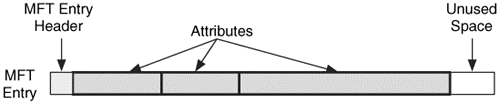
\includegraphics[scale=0.6]{figuras/fig02.png}
  \caption{Entrada na MFT - Cabe�alho e espa�o reservado aos diferentes tipos de atributos. Para o exemplo, a entrada possui 3 atributos.}
  \label{fig:fig02}
\end{figure}

\section{Aloca��o de Arquivos}
...

\section{An�lise NTFS}
...